\subsection{Reads and Writes}
\label{sec:readwrite}
There are two operations that are issued by the driver --- read and write.
The driver keeps track of the most recent version for each replica in a list.
This structure is updated on a write and used to decide which replica to 
request a read from.

Figure~\ref{fig:write} shows the message flow on a write request. Notice
that we utilize chained replication, where the closer the replica is to the 
head of the chain the more more up-to-date it is. The choice for this chained
scheme is to reduce the network load to the driver. Thus, when 
the driver sends a write request, \texttt{sdaemon} issues the write to its 
local LSVD copy and then propagates the request to the next replica in the 
chain. After writing to its own LSVD, each replica sends back a response to
the driver with a status and its current version number. The driver then 
updates its replica list with the version in the sent response. If a majority
of replicas responds to the driver with a SUCCESS message, then the driver 
reports a success back to the kernel. Otherwise, it will report a failure. 

In contrast, a read only needs one replica to respond for a success. In 
Figure~\ref{fig:read} we observe that when the driver issues a read request 
it issues the request to the replica with the most recent version. Typically 
this is the primary replica. If the replica responds with a SUCCESS, then 
the driver serves the request back to the kernel. Otherwise, it will issue 
the request to the next replica in the chain with the most recent version. I 
no replicas respond, then the driver reports a failure.

\begin{figure}[t]
    \begin{subfigure}{0.5\textwidth}
        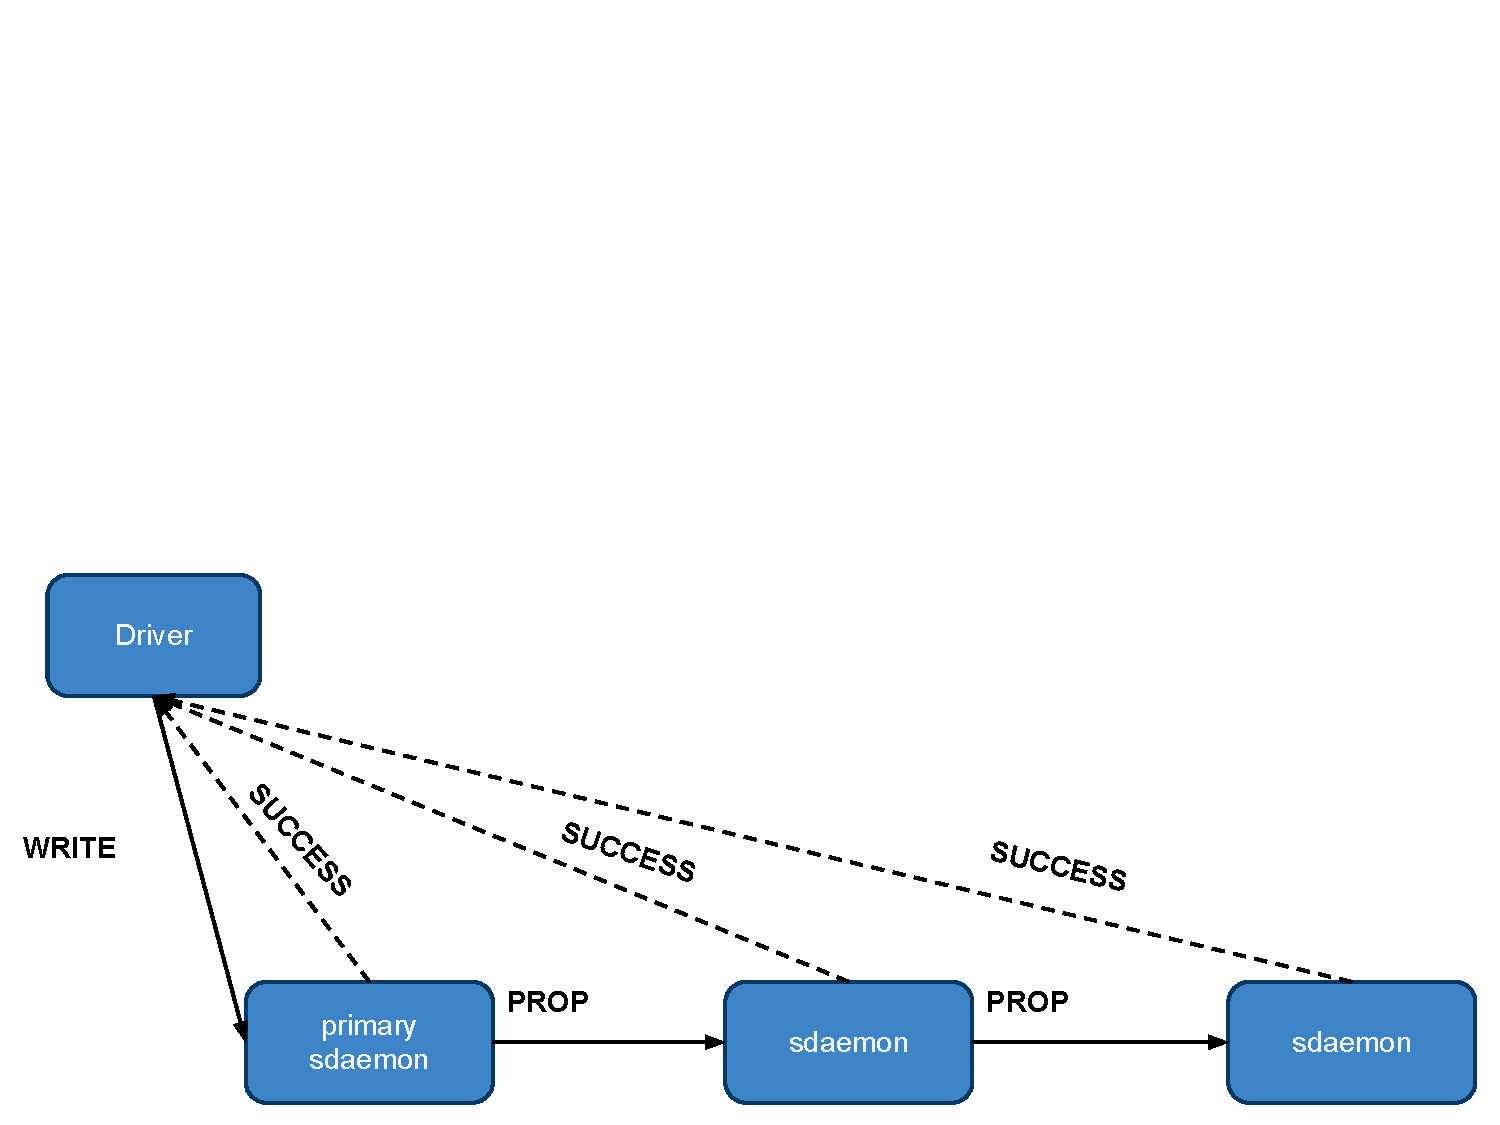
\includegraphics[width=\textwidth, trim=0 0 0 3.5in, clip]{./figures/write.pdf}
        \caption{The message flow for a write operation. A quorum of SUCCESS 
                 responses must be received for a successful write.}
        \label{fig:write}
    \end{subfigure}
    ~
    \begin{subfigure}{0.5\textwidth}
        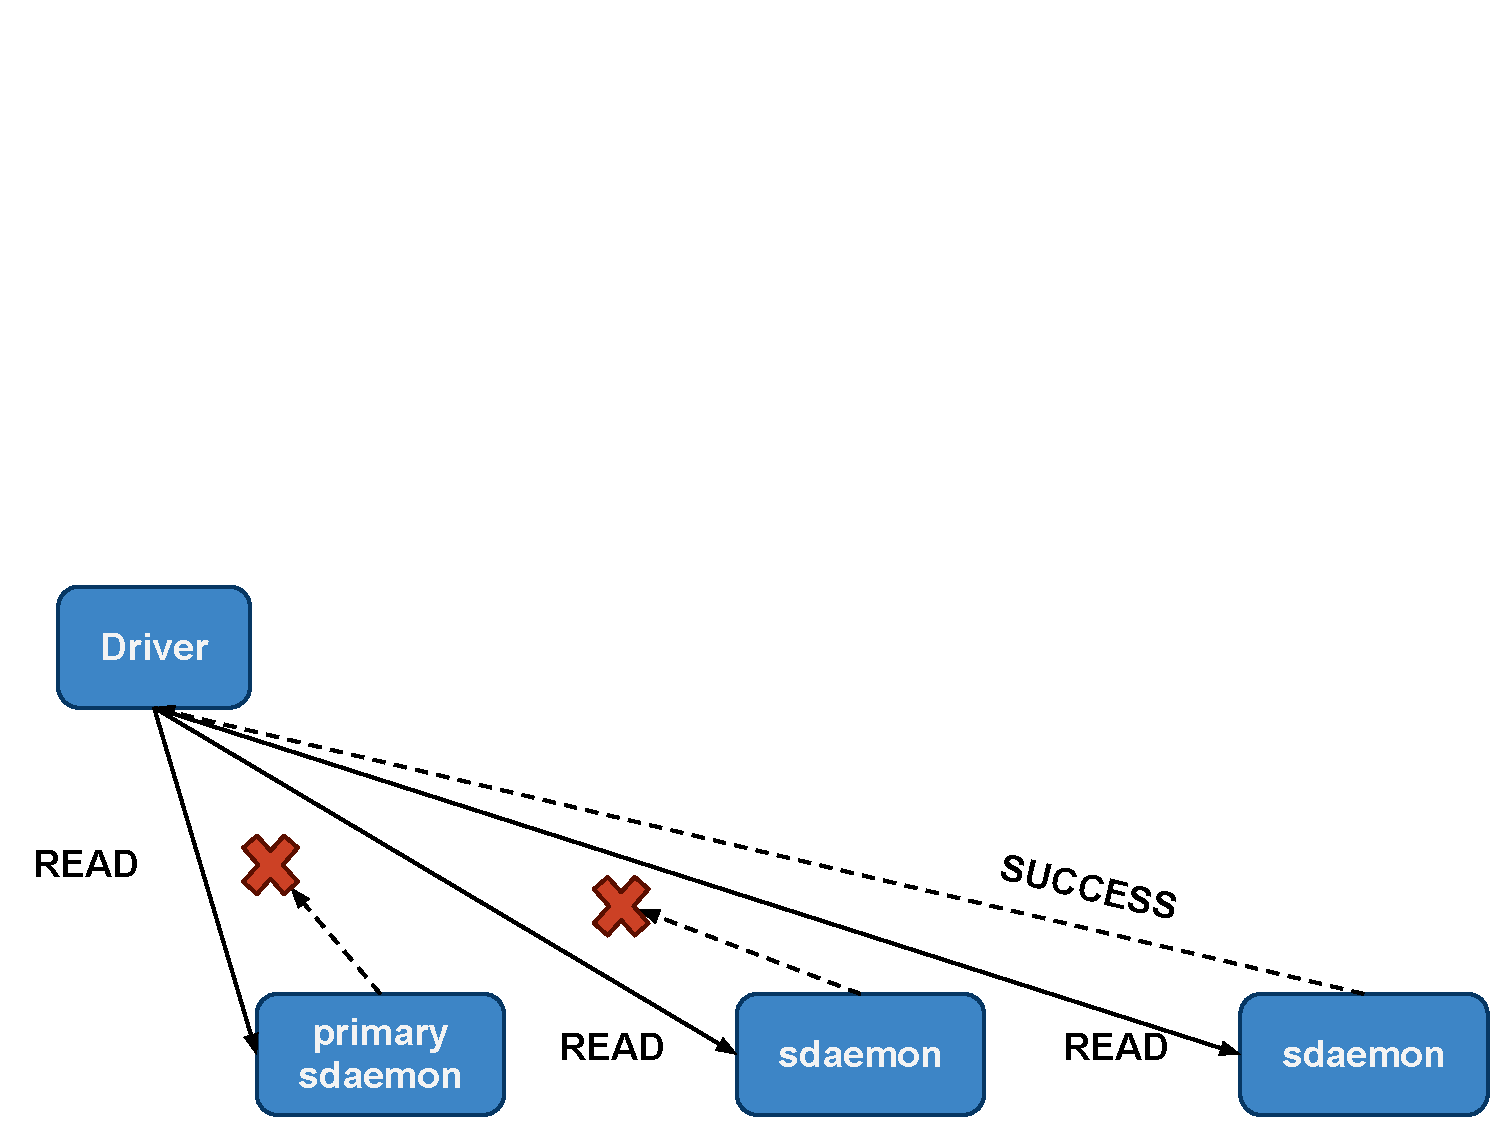
\includegraphics[width=\textwidth, trim=0 0 0 3.5in, clip]{./figures/read.pdf}
        \caption{The message flow for a read operation. A read request is 
            issued to the replica with the most recent version until a 
            SUCCESS is received or if no replicas with the most recent 
            version responds with SUCCESS.}
        \label{fig:read}
    \end{subfigure}
    \caption{Message flows for read and write operations}
\end{figure}

\subsection{Replication}
\label{sec:replication}
Replication is managed by \texttt{sdaemon} using write propagation and 
synchronization. Propagation was discussed in Section~\ref{sec:readwrite}. 
Synchronization is performed whenever a replica joins the chain and also 
periodically to keep replicas near the tail from becoming increasingly out 
of date. Figure~\ref{fig:sync} shows how replication is performed. As we see,
replica C sends a SYNC request with the version number of its local LSVD 
copy to the previous replica in the chain, replica B. Replica B then responds
with all the writes from C.version to B.version. Replica C then applies all 
the writes to its LSVD. After the synchronization operation, Replica C's 
LSVD version is equal to B's version. Similarly, replica B initiates the 
synchronization procedure with replica A.

To handle failure, a replica controller is used to inform the driver and 
neighboring replicas that a failure has occured. This controller keeps track 
of the liveliness of each replica by recording the elapsed time since the 
last heartbeat message, which is sent every $T$ seconds by each replica. After
$2T$ seconds the controller flags the replica as \emph{inactive} and after 
$4T$ seconds the replica is marked as failed. Upon failure, the controller 
informs the kernel and the neighboring replicas using update messages. Upon
receipt of the update messages, the two neighboring replicas connect to each
other. The latter replica sends a SYNC request, and then normal operation 
resumes. Meanwhile, the controller spins off a new \texttt{sdaemon} process
that is appended to the end of the chain. Note that currently the replica 
controller is not implemented.

\begin{figure}[t]
    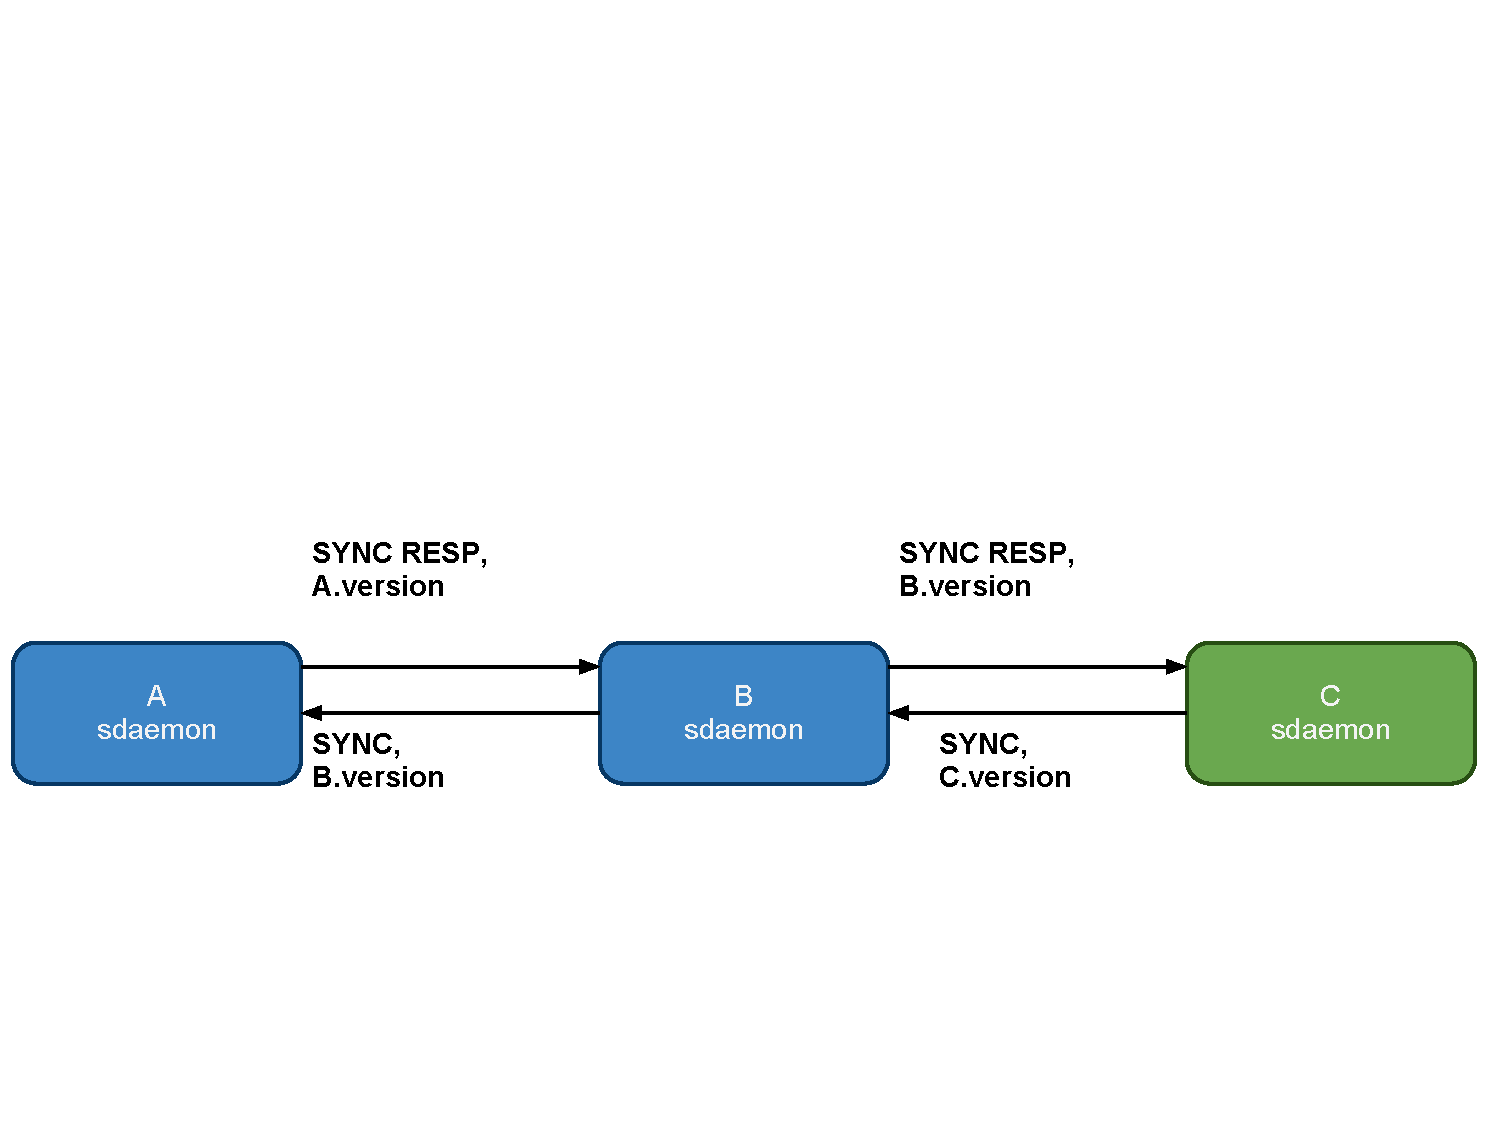
\includegraphics[width=0.45\textwidth, trim=0 2in 0 3in, clip]{./figures/sync.pdf}
    \caption{The message flow for a synchronization operation. Replica C 
            sends a SYNC request to its predecessor, which responds with all
            the writes since C's version.}
    \label{fig:sync}
\end{figure}

\subsection{Log Structured Virtual Disk}
\label{sec:lsvd}

When designing our file format to back virtual disk, we had few goals in mind. First, the file should be dynamically growing. If a disk was defined with $D$ bytes free space and user is using only $C$ bytes for his content, the backing file size should use $O(C)$ bytes. Second, we have to support versioning. We define version as update sequence number. Each update increments disk version by one. To enable synchronization, storage deamon has to be aware of the current local disk version and has to be able to send arbitrary version updates to other replicas for synchronization. Third goals was consistency. If the local data has version $V$, it should include all updates with versions less than or equal to $V$ and none of the updates with versions bigger than $V$. Finally, our fourth goal was ability to easily support snapshots and incremental backups.

To address all these requirements, we developed Log Structured Virtual Disk (LSVD). When we receive updates, we just write them sequentially on a disk and increment version number by one. That way, we are dynamically growing. We also support versioning and are consistent, since we remember all updates together with their version number. Finally, it is easy to support snapshoting and incremental backups. On snapshot operation, we just create new file and use old file as a base. New updates go to the new file and we can read old data from old, read-only base file.

Figure \ref{fig:lsvd} shows the actual data layout in LSVD file. First few bytes define the superblock, which contains important metadata. Next, there are two checkpointing placeholders. After that, actual updates are layed out. Each update consists of data block and commit block. Data block can hold one or more sectors. Io our implementation, we use 4KB sector sizes. Commit block verifies integrity of the data block by storing its checksum. To be able to guarantee consistency, we need to have atomic version writes. If a commit block is not written to disk or checksum is invalid, we define the update as not commited.

On a write, we just append write to the end of the file with additional metadata. On a read, therefore, we need to be able to find requested sectors on the disk. For that, we keep in-memory \emph{sector to offset map}. It maps disk sectors to file offsets where the sector's data is stored. On every write, we easily update the map. When opening a disk after recovery, we are able to rebuild sector to offset map by reading all the updates from the beginning of time. That would, however, be very slow. To keep recovery time from growing linearly with time, we do \emph{checkpointing}. Every 60 seconds, we write the sector to offset map to disk into one of the checkpointing placeholders at the beginning of the file. We execute checkpointing writes slowly. That way, we do not slow down regular write or read operations, especially since checkpointing writes are random writes. Superblock keeps a pointer to an active checkpoint. After the checkpoint is fully written to one of the placeholders, we update the superblock and \texttt{fsync}. During recovery, checkpoint is loaded into memory and recovery continues from the point in time when checkpoint was started. That way, we limit recovery time and keep it from not growing linearly with time.

\begin{figure}[h]
    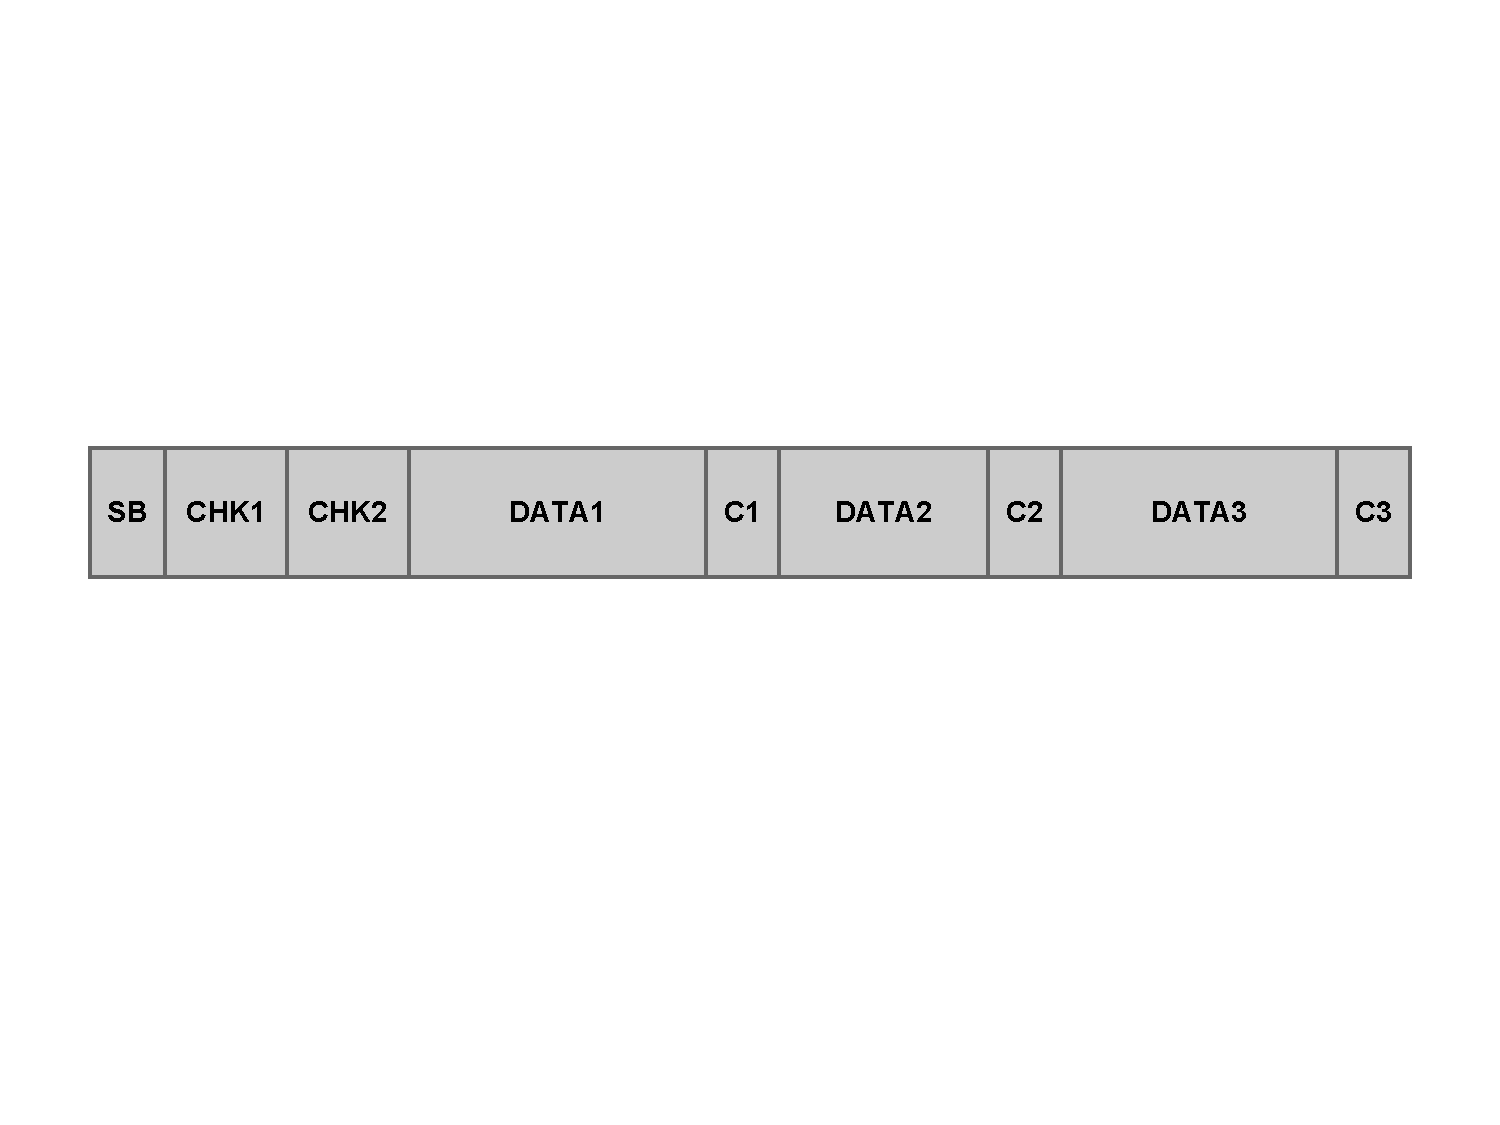
\includegraphics[width=0.45\textwidth]{./figures/lsvd.pdf}
    \caption{The LSVD file structure.}
    \label{fig:lsvd}
\end{figure}

\emph{Discussion on how versioning works, how we can retrieve arbitrary 
writes (change logs?) how we can easily extend this framework for snapshotting.}
